\section{Experimental Studies}\label{sec:experiments}
\subsection{Test Instances and Evaluation Protocol}
The experiments use synthetic inputs from a seeded generator. They do not represent measured industrial products. The main set contains three seeds, 32--34, at two configurations: 80 tasks on four lines and 120 tasks on six lines. Each line has 20 tasks and eight candidate stations. Both methods read the same frozen input bytes. The task graph is layered and contains only within-line forward arcs. Required tasks occupy the first 20\% of each line's task list. Recovery requires at least 35\% of the total task weight, rounded upward.

The generator samples mode availability and task economics before partitioning the task bank. It provides a structurally feasible construction for input checks. Neither solver receives this construction as an initial solution. Shared capacities in the main set equal the observed independent economic calibration counts minus one for each resource. This calibration defines a development design, not a random industrial population. The supplementary file provides the generator rules and all capacity values.

A second set retains the 120-task inputs and sets each shared capacity to the ceiling of 80\% of its calibrated independent use. A retained 80-task two-line input provides a large-block boundary. A separate structure study compares two, four, and eight lines at 80 total tasks. Repartitioning retains the task bank but changes precedence graphs and recovery rows. These are different mathematical inputs. The study therefore does not isolate line count as the only causal factor.

The direct baseline solves the compact MILP with CPLEX. The decomposition also uses CPLEX inside line pricing, profile queries, and integer recovery. All measured pairs use the same machine, CPLEX~22.1.1, one thread, random seed~11, and zero requested MIP gap. The archived environment contains Python~3.10.11, PuLP~3.3.2, and Windows~10. The physical processor model is not preserved in the archived environment and requires confirmation for submission.

The main protocol allocates 600 seconds per method. The resource-constrained protocol allocates 180 seconds. Both reserve five seconds for evidence finalization. A parent process measures execution from worker startup through exit, including required result persistence. Independent offline replay is separate. The watchdog and native solver limits operate under Windows scheduling; the protocol is not a hard real-time guarantee. All listed main and robustness workers return timely, complete evidence. A time-limited CPLEX completion time is censored. It is not an observed time to optimality. No 3600-second run enters these tables.

\subsection{Parameters and Performance Metrics}
The framework uses a 0.5-second economic initialization per line and a 0.5-second feasibility fallback when necessary. Restricted integer recovery receives up to 0.5 seconds per call. CG receives at most 90\% of the available internal budget. The pricing loop divides remaining time among the remaining lines. Initial profile queries receive up to two seconds. Repeated attempts double that allowance, subject to the remaining global time. The maximum CG record count is 100. These settings are fixed for the reported main and resource-constrained sets. They are implementation settings, not parameters inferred from a cited study.

The LP primal and dual tolerances are $10^{-8}$. Pricing integrality, reduced-cost, and artificial tolerances are $10^{-7}$. Original-solution verification uses $10^{-6}$. Bound consistency and absolute integer closure use $10^{-5}$. Relative integer closure uses $10^{-8}$. The supplementary file lists all numerical roles.

The primary metrics are the validated integer LB, valid UB, gap in \eqref{eq:gap}, integer proof state, and measured execution time. Additional metrics include pricing calls, generated columns, Phase I and II pricing rounds, and native solver time. A round count excludes RMP-only phase transitions and early closure records. Compact-model search nodes and CG rounds represent different operations and are not directly compared.

\subsection{Feasibility and Integer-Certificate Checks}
Small instances use an independent enumerator of task omission, station assignment, and allowed mode. The enumerator checks task selection, AND precedence, time, fatigue, deployment, and recovery directly from data. An independently assembled complete-column LP and integer model provide reference values. Archived checks also compare CPLEX and CBC on these small cases.

\begin{table}[!t]\centering\small
\caption{Small Complete-Column Checks}\label{tab:small}
\setlength{\tabcolsep}{3pt}
\begin{tabular}{lrrl}\toprule
Case & Line LP & Full integer & Profile result\\\midrule
Five-task reference &24.00&24.00&Optimal\\
Six-task reference &56.63&56.63&Optimal\\
Positive-gap case &6.50&2.00&Optimal\\
LP-feasible/IP-infeasible &4.00&Infeasible&Infeasible\\\bottomrule
\end{tabular}
\end{table}
Table~\ref{tab:small} confirms the need to distinguish LP and integer conclusions. The positive-gap case requires integer coordination despite exact CG convergence. The LP-feasible/IP-infeasible case contains no integer witness. Resource-profile analysis proves its integer infeasibility. These small archived tests establish implementation consistency within their enumerated scope. They do not replace larger-instance performance evaluation.

\subsection{Illustrative Task Assignment}
Fig.~\ref{fig:gantt} illustrates the framework's solution for an additional 20-task synthetic instance with two lines and four candidate stations per line. Both the framework and Compact CPLEX certify an optimal profit of 132.58. The displayed plan selects 14 tasks and deploys three human resources and two robots. Task-to-station assignments and execution modes come from the verified integer solution; the displayed within-station order is reconstructed by a precedence-compatible topological sort. Each row uses its own station-cycle clock, rather than a single product's end-to-end timeline.

\begin{figure*}[!tp]\centering
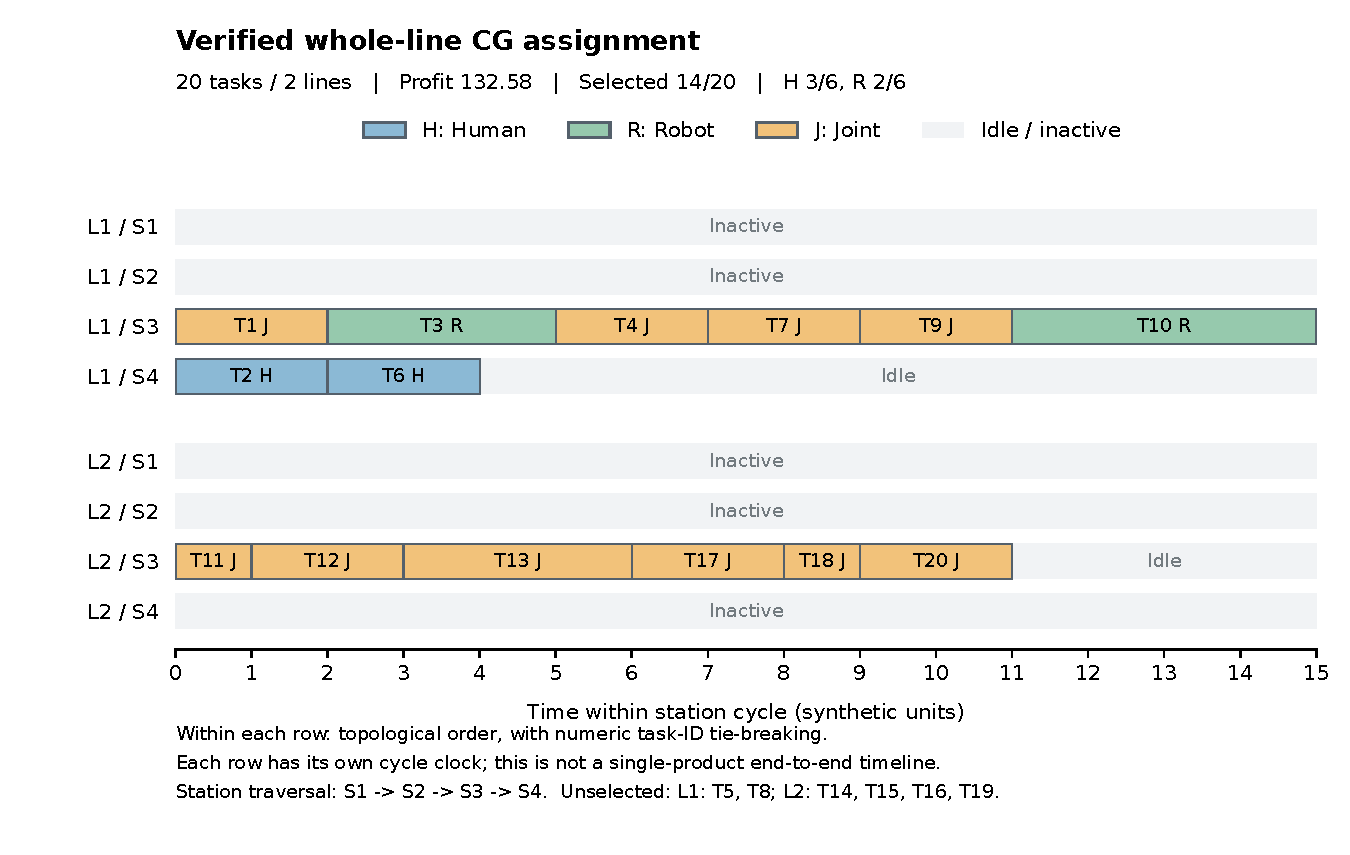
\includegraphics[width=0.90\textwidth]{img/gantt_assignment.pdf}
\caption{Illustrative task allocation on two disassembly lines with a cycle time of 15 synthetic time units. Bars identify tasks and execution modes: H (human), R (robot), and J (joint). Gray intervals show idle time or inactive stations. The reconstructed local order respects within-station precedence; it is not an optimized start-time schedule.}\label{fig:gantt}
\end{figure*}

\subsection{Main Comparison With Compact CPLEX}
\input{tables/formal}
Table~\ref{tab:formal} shows an integer-certification advantage on all six main inputs. The framework establishes optimality in 19.36--182.69 seconds. Compact CPLEX remains unproven within the 600-second protocol. On the three 80-task inputs, both methods reach the same final integer profit. Their difference concerns proof completion. On two 120-task inputs, the framework also returns a higher final integer profit. On seed~34, Compact CPLEX reaches the same profit but retains a positive bound gap.

\begin{figure*}[!t]\centering
\includegraphics[width=\textwidth]{img/performance_lines.pdf}
\caption{All six paired main inputs, ordered by total tasks and seed: (a) recorded end-to-end time; (b) final certified relative gap. Open triangles indicate time-limited, unproven compact results; filled circles indicate completed decomposition integer proofs. Compact times are censored observations, not times to optimality. Lines connect distinct inputs only as visual guides; they are not convergence trajectories.}\label{fig:runtime}
\end{figure*}
Fig.~\ref{fig:runtime} presents the same comparisons without converting cutoffs into exact speedup ratios. These results support efficient certification on the tested multi-line configurations. They do not establish that the framework first discovers an optimal-profit plan earlier. Comparable first-optimum timestamps are not available for Compact CPLEX.

\subsection{Resource Coordination and a Large-Block Boundary}
\input{tables/robust}
Table~\ref{tab:robust} extends the comparison to stronger resource competition. The framework proves the three 120-task optima under the 180-second protocol. Compact CPLEX remains unproven and returns lower profits. Seeds~32 and~33 close through verified integer plans and complete CG bounds. Seed~34 requires 31 demand-driven profile queries after an incomplete CG pricing round. Its final certificate concerns the original integer optimum. It does not assert complete line-LP convergence.

The two-line case in Table~\ref{tab:robust} provides a contrary result. Two lines with 40 tasks each produce difficult local MILPs. The decomposition returns both a lower profit and a looser UB than Compact CPLEX. Its CG pricing consumes about 156 seconds, and subsequent profile queries do not close the gap. Thus total task count alone does not predict the benefit of decomposition.

The separate 80-task structure study provides further context. A resource-constrained eight-line input reaches the same proven optimum under both methods. The framework completes in about 2.91 seconds; Compact CPLEX completes in about 128.09 seconds. A resource-ample eight-line input instead favors Compact CPLEX, at about 1.24 versus 1.64 seconds. The supplementary tables retain every compact/decomposition pair in that structure study. The evidence supports a tradeoff between block difficulty and coordination, rather than a universal benefit from adding lines.

\subsection{Iterations, Cost, and Interpretation}
\input{tables/iterations}
Table~\ref{tab:iterations} shows that Phase II needs only three to five pricing rounds in the main experiment. Native pricing nevertheless accounts for about 91--99\% of total framework time. Each RMP uses less than 0.01 second of native solve time. The restricted integer master also remains small. These observations identify local pricing difficulty as the main cost in this regime.

The whole-line formulation can strengthen the relaxation through local integer convexification. It can also simplify integer combination by placing all within-line compatibility inside each column. The experiments are consistent with these mechanisms. They do not isolate relaxation strength from warm-start behavior or solver search-state effects. A full component ablation is still required to quantify each contribution.

The evaluation has a defined boundary. It uses a small synthetic development suite and one solver seed per measured input. Resource calibration is part of the instance construction. The suite does not establish statistical significance, industrial ergonomic validity, or performance on arbitrary large line blocks. Broader comparator algorithms, measured product cases, and an independent final test suite remain necessary before a broad state-of-the-art claim.
